% How to use writeLaTeX: 
%
% You edit the source code here on the left, and the preview on the
% right shows you the result within a few seconds.
%
% Bookmark this page and share the URL with your co-authors. They can
% edit at the same time!
%
% You can upload figures, bibliographies, custom classes and
% styles using the files menu.
%
% If you're new to LaTeX, the wikibook is a great place to start:
% http://en.wikibooks.org/wiki/LaTeX
%
%%%%%%%%%%%%%%%%%%%%%%%%%%%%%%%%%%%%%%%%%%%%%%%%%%%%%%%%%%%%%%%%%%%%%%
% Edit the title below to update the display in My Documents
%\title{Project Report}
%
%%% Preamble
\documentclass[paper=a4, fontsize=11pt]{scrartcl}
\usepackage[T1]{fontenc}
\usepackage{fourier}

\usepackage[english]{babel}     % English language/hyphenation
\usepackage[protrusion=true,expansion=true]{microtype}	
\usepackage{verbatim}
\usepackage{amsmath,amsfonts,amsthm} % Math packages
\usepackage[pdftex]{graphicx}
\graphicspath{ {images/} }
\usepackage{url}

%%% Custom margins
\usepackage[hscale=0.75,vscale=0.75,vmarginratio={4:5},heightrounded]{geometry}

%%% Custom sectioning
\usepackage{sectsty}
\allsectionsfont{\centering \normalfont\scshape}

%%% Custom headers/footers (fancyhdr package)
\usepackage{fancyhdr}
\pagestyle{fancy}
\fancyhead{}											% No page header
\fancyfoot[L]{}											% Empty 
\fancyfoot[C]{}											% Empty
\fancyfoot[R]{\thepage}									% Pagenumbering
\renewcommand{\headrulewidth}{0pt}			% Remove header underlines
\renewcommand{\footrulewidth}{0pt}				% Remove footer underlines
\setlength{\headheight}{13.6pt}


%%% Equation and float numbering
\numberwithin{equation}{section}		% Equationnumbering: section.eq#
\numberwithin{figure}{section}			% Figurenumbering: section.fig#
\numberwithin{table}{section}				% Tablenumbering: section.tab#
\setlength{\parskip}{5pt}

%%% Maketitle metadata
\newcommand{\horrule}[1]{\rule{\linewidth}{#1}} 	% Horizontal rule

\title{
		%\vspace{-1in} 	
		\usefont{OT1}{bch}{b}{n}
		\normalfont \normalsize \textsc{CSCI 580, Prof. Saty Raghavachary} \\ [25pt]
		\horrule{0.4pt} \\[0.5cm]
		\huge\textbf{Crepescular Rays using Ray Tracing} \\
		\vspace{10pt}
		\normalsize\textbf{Team Uncanny Valley}
		\horrule{0.4pt} \\[0.5cm]
}
\author{
		\normalfont\normalsize
        Sanskriti Lastname, Saurabh Mistry, Sreepada Rao Singeetham, Tushar Tiwari\\[-3pt]		\normalsize
        \today
}
\date{}

%%% Begin document
\begin{document}
\maketitle
\begin{center}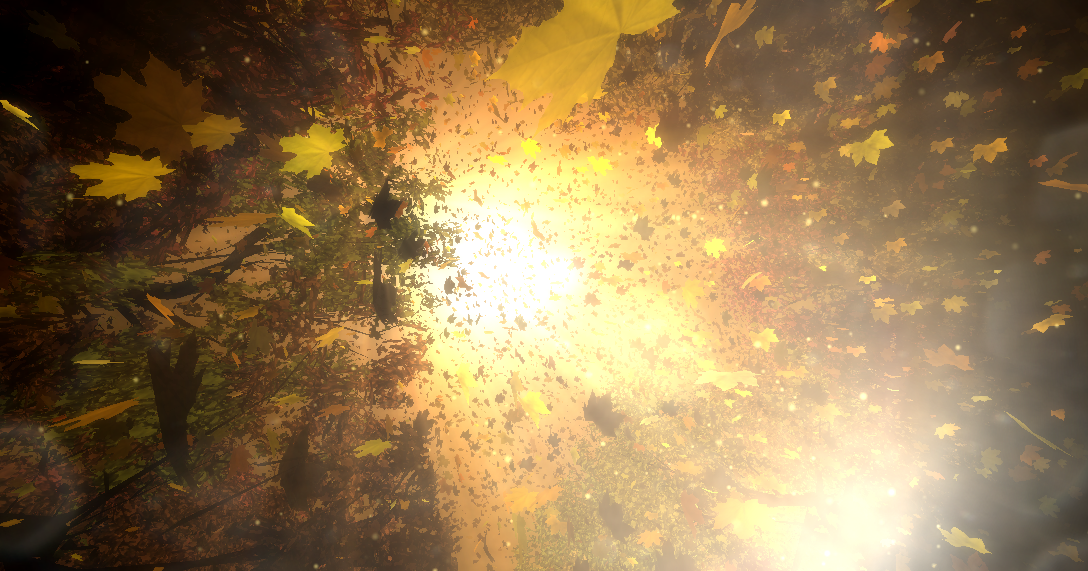
\includegraphics[width=\textwidth]{Title}\end{center}
\section{Objective}
To achieve the above render, we make use of two well-known techniques namely Ray Tracing and Volumteric Lighting. Ray Tracing is a technique for generating an image by tracing the path of light. Volumetric Lighting is a technique that allows the viewer to see beams of light called crepescular rays.
\newpage
\fancyhf{}
\fancyhead[RE,LO]{Crepescular Rays}
\fancyhead[LE,RO]{Introduction}
\fancyfoot[CE,CO]{\leftmark}
\fancyfoot[LE,RO]{\thepage}
\renewcommand{\headrulewidth}{1pt}
\renewcommand{\footrulewidth}{1pt}
\section{Introduction}
The Ray Tracing algorithm very much mimics the procedure of observing the color of an object in nature. A light source emits a ray of light which travels, eventually, to a surface that interrupts its progress. One can think of this "ray" as a stream of photons traveling along the same path. There are two basic ideas for ray tracing.
\par
Forward ray tracing and backward ray-tracing. Forward ray-tracing is how the color of an object is observed by the eye in real life. That is, a ray of light is reflected of an object and travels into the eye producing an image. However, this algorithm is impractical because there will be many rays that will miss the camera and will not be useful to us. Thus, there will be a huge computational overhead. 
\par
For CG purposes, we make use of the backward ray-tracing algorithm. The basic idea is shoot a ray from the camera through each pixel of the image plane. If this ray intersects with an object, we send out another ray in the direction of our light source to determine if the object is under a shadow of another object. We also send out a reflected ray to obtain the reflection of another object if the object is capable of reflections.
\vspace{20pt}
\begin{center}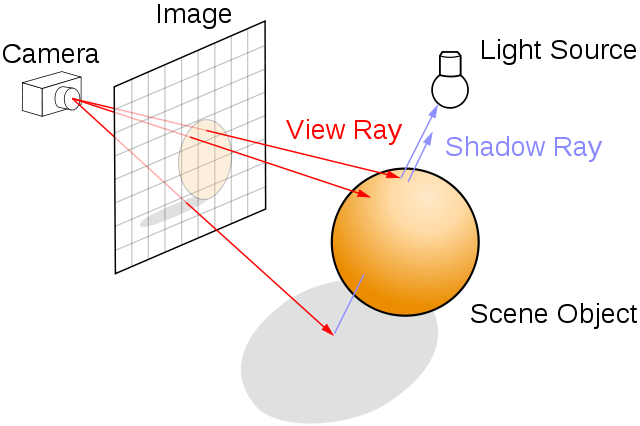
\includegraphics[width=\textwidth]{ray_tracing_wiki}\end{center}
\newpage
\section{Implementation}
\subsection{Scene Creation and Obj Format}
Since most objs out there use the v, vt, f and quadrilateral format, our program had to be modified to read data in that format and modify it into triangles.
\par
Moreover, a single leaf obj wouldn't suffice for the purposes of this project. So we took the same leaf obj, randomly translated it, rotated it and scaled it to create a scene that represented falling leaves. All these combinations of leaves in different orientations were merged into one singe obj file that could now depict the whole screen.

\subsection{Backward Ray Tracing}

%%%\begin{itemize}
	%%%\item Compute the Viewing Rays
\subsubsection{Compute the Camera Rays}
We represent a ray by obtaining the ray's origin and its direction. The first ray we look at is the viewing or camera ray. This ray is computed by making use of the camera position and the current pixel which has to be coloured. We first transform the pixel coordinates to $x, y \in [-1, 1]$.
\[ i = \dfrac{x * 2}{imagePlaneWidth} - 1 \]
\[ j = \dfrac{y * 2}{imagePlaneHeight} - 1 \]

The ray line equation can be written as:
\[Some stuff.\]

\subsubsection{Compute the intersection of the camera ray\\ with the plane of the triangle}
Since there is no way knowing which triangle the ray will intersect with, we have to try out all triangles.
To check if the ray intersects with the plane of the triangle is easy. By finding out the normal to the triangle and taking the dot product of the ray and this normal we can verify if the triangle is parallel to the ray or starts behind the triangle or neither of those. 
\par
To begin with we need to make sure that we get the normal outwards rather than inwards. This will ensure that we get the correct normals. We first arrange all vertices in a counter-clockwise manner. If $v_{0}, v_{1} and v_{2}$ are the vertices in counter-clockwise order, then the normal is obtained by,
\[_{n} = \overrightarrow{(v_{1}-v_{0})} \times \overrightarrow{(v_{2}-v_{0})}\]
\[\bigtriangleup _{normal} = \hat{n} = \dfrac{n}{\lvert n \rvert}\]

Then the dot product of the $\bigtriangleup _{normal}$ and the ray can provide us with information whether the $\bigtriangleup$ is parallel to the ray or not.
\[ \bigtriangleup _{normal} \cdot \overrightarrow{r_{c}}\ = 0 \implies \bigtriangleup \parallel \overrightarrow{r_{c}}\]
\[ \bigtriangleup _{normal} \cdot \overrightarrow{r_{c}}\ < 0 \implies \bigtriangleup is behind \overrightarrow{r_{c}}\]
\[ \bigtriangleup _{normal} \cdot \overrightarrow{r_{c}}\ > 0 \implies \bigtriangleup  \not\parallel \overrightarrow{r_{c}}\]

We are interested in the last condition because this signifies that the camera ray intersects the plane of the $\bigtriangleup$.

\subsubsection{Check if intersection point is inside the Triangle}
To obtain the point of intersection we must first compute the triangle distance:
\[d(\bigtriangleup) = \bigtriangleup_{normal} \cdot v_{0}\]
Then, the following equation gives us the distance to the plane:
\[d(plane) = -1 \times \dfrac{\bigtriangleup_{normal} \cdot (\overrightarrow{r_{c}} + (\bigtriangleup_{normal} \times -d(\bigtriangleup)))}{\bigtriangleup_{normal}\cdot \overrightarrow{r_{c}}}  \]
Next we need to find the point that intersects with the plane.
This point, say $q$, is found by:
\[q = d(plane)\cdot\overrightarrow{r_{c}} + r_{c}\]
Now, that we have the point, we need to verify if this point lies inside the $\bigtriangleup$.
\[\dfrac{Area(q, v_{1}, v_{2}) + Area(q, v_{0}, v_{2}) + Area(q, v_{0}, v_{1})}{Area(v_{0}, v_{1}, v_{2})} \approx 1\]
If the above condition holds then our point is inside the $\bigtriangleup$.

\subsection{Volumetric Shadows}

\subsection{Lens Flare}
We made use of an image downloaded from the internet. This image was drawn over the canvas to obtain the lens-flare effect.
\section{Challenges}
\begin{itemize}
\item One of the biggest challenges in the project is the slow computation time of ray tracing. Since every pixel is rendered against every triangle in the scene. The computation time is very huge.
\item We were stuck at one point when finding whether the point on the ray-plane intersection is inside or outside the triangles. We had to try various ways to get the ray tracing working.
\end{itemize}
\section{Conclusion}
While researching and implementing Ray-Tracing we were exposed to many methods that showed us how to implement photorelaistic images. We were also made aware of the enormous computations done in the ray-tracing algorithm. We also investigated several ways to check if the point exists in the triangle or not.

\section{References}
%Add references
\begin{itemize}
\item 
\end{itemize}

%%% End document
\end{document}